
% Default to the notebook output style

    


% Inherit from the specified cell style.




    
\documentclass[11pt]{article}

    
    
    \usepackage[T1]{fontenc}
    % Nicer default font (+ math font) than Computer Modern for most use cases
    \usepackage{mathpazo}

    % Basic figure setup, for now with no caption control since it's done
    % automatically by Pandoc (which extracts ![](path) syntax from Markdown).
    \usepackage{graphicx}
    % We will generate all images so they have a width \maxwidth. This means
    % that they will get their normal width if they fit onto the page, but
    % are scaled down if they would overflow the margins.
    \makeatletter
    \def\maxwidth{\ifdim\Gin@nat@width>\linewidth\linewidth
    \else\Gin@nat@width\fi}
    \makeatother
    \let\Oldincludegraphics\includegraphics
    % Set max figure width to be 80% of text width, for now hardcoded.
    \renewcommand{\includegraphics}[1]{\Oldincludegraphics[width=.8\maxwidth]{#1}}
    % Ensure that by default, figures have no caption (until we provide a
    % proper Figure object with a Caption API and a way to capture that
    % in the conversion process - todo).
    \usepackage{caption}
    \DeclareCaptionLabelFormat{nolabel}{}
    \captionsetup{labelformat=nolabel}

    \usepackage{adjustbox} % Used to constrain images to a maximum size 
    \usepackage{xcolor} % Allow colors to be defined
    \usepackage{enumerate} % Needed for markdown enumerations to work
    \usepackage{geometry} % Used to adjust the document margins
    \usepackage{amsmath} % Equations
    \usepackage{amssymb} % Equations
    \usepackage{textcomp} % defines textquotesingle
    % Hack from http://tex.stackexchange.com/a/47451/13684:
    \AtBeginDocument{%
        \def\PYZsq{\textquotesingle}% Upright quotes in Pygmentized code
    }
    \usepackage{upquote} % Upright quotes for verbatim code
    \usepackage{eurosym} % defines \euro
    \usepackage[mathletters]{ucs} % Extended unicode (utf-8) support
    \usepackage[utf8x]{inputenc} % Allow utf-8 characters in the tex document
    \usepackage{fancyvrb} % verbatim replacement that allows latex
    \usepackage{grffile} % extends the file name processing of package graphics 
                         % to support a larger range 
    % The hyperref package gives us a pdf with properly built
    % internal navigation ('pdf bookmarks' for the table of contents,
    % internal cross-reference links, web links for URLs, etc.)
    \usepackage{hyperref}
    \usepackage{longtable} % longtable support required by pandoc >1.10
    \usepackage{booktabs}  % table support for pandoc > 1.12.2
    \usepackage[inline]{enumitem} % IRkernel/repr support (it uses the enumerate* environment)
    \usepackage[normalem]{ulem} % ulem is needed to support strikethroughs (\sout)
                                % normalem makes italics be italics, not underlines
    

    
    
    % Colors for the hyperref package
    \definecolor{urlcolor}{rgb}{0,.145,.698}
    \definecolor{linkcolor}{rgb}{.71,0.21,0.01}
    \definecolor{citecolor}{rgb}{.12,.54,.11}

    % ANSI colors
    \definecolor{ansi-black}{HTML}{3E424D}
    \definecolor{ansi-black-intense}{HTML}{282C36}
    \definecolor{ansi-red}{HTML}{E75C58}
    \definecolor{ansi-red-intense}{HTML}{B22B31}
    \definecolor{ansi-green}{HTML}{00A250}
    \definecolor{ansi-green-intense}{HTML}{007427}
    \definecolor{ansi-yellow}{HTML}{DDB62B}
    \definecolor{ansi-yellow-intense}{HTML}{B27D12}
    \definecolor{ansi-blue}{HTML}{208FFB}
    \definecolor{ansi-blue-intense}{HTML}{0065CA}
    \definecolor{ansi-magenta}{HTML}{D160C4}
    \definecolor{ansi-magenta-intense}{HTML}{A03196}
    \definecolor{ansi-cyan}{HTML}{60C6C8}
    \definecolor{ansi-cyan-intense}{HTML}{258F8F}
    \definecolor{ansi-white}{HTML}{C5C1B4}
    \definecolor{ansi-white-intense}{HTML}{A1A6B2}

    % commands and environments needed by pandoc snippets
    % extracted from the output of `pandoc -s`
    \providecommand{\tightlist}{%
      \setlength{\itemsep}{0pt}\setlength{\parskip}{0pt}}
    \DefineVerbatimEnvironment{Highlighting}{Verbatim}{commandchars=\\\{\}}
    % Add ',fontsize=\small' for more characters per line
    \newenvironment{Shaded}{}{}
    \newcommand{\KeywordTok}[1]{\textcolor[rgb]{0.00,0.44,0.13}{\textbf{{#1}}}}
    \newcommand{\DataTypeTok}[1]{\textcolor[rgb]{0.56,0.13,0.00}{{#1}}}
    \newcommand{\DecValTok}[1]{\textcolor[rgb]{0.25,0.63,0.44}{{#1}}}
    \newcommand{\BaseNTok}[1]{\textcolor[rgb]{0.25,0.63,0.44}{{#1}}}
    \newcommand{\FloatTok}[1]{\textcolor[rgb]{0.25,0.63,0.44}{{#1}}}
    \newcommand{\CharTok}[1]{\textcolor[rgb]{0.25,0.44,0.63}{{#1}}}
    \newcommand{\StringTok}[1]{\textcolor[rgb]{0.25,0.44,0.63}{{#1}}}
    \newcommand{\CommentTok}[1]{\textcolor[rgb]{0.38,0.63,0.69}{\textit{{#1}}}}
    \newcommand{\OtherTok}[1]{\textcolor[rgb]{0.00,0.44,0.13}{{#1}}}
    \newcommand{\AlertTok}[1]{\textcolor[rgb]{1.00,0.00,0.00}{\textbf{{#1}}}}
    \newcommand{\FunctionTok}[1]{\textcolor[rgb]{0.02,0.16,0.49}{{#1}}}
    \newcommand{\RegionMarkerTok}[1]{{#1}}
    \newcommand{\ErrorTok}[1]{\textcolor[rgb]{1.00,0.00,0.00}{\textbf{{#1}}}}
    \newcommand{\NormalTok}[1]{{#1}}
    
    % Additional commands for more recent versions of Pandoc
    \newcommand{\ConstantTok}[1]{\textcolor[rgb]{0.53,0.00,0.00}{{#1}}}
    \newcommand{\SpecialCharTok}[1]{\textcolor[rgb]{0.25,0.44,0.63}{{#1}}}
    \newcommand{\VerbatimStringTok}[1]{\textcolor[rgb]{0.25,0.44,0.63}{{#1}}}
    \newcommand{\SpecialStringTok}[1]{\textcolor[rgb]{0.73,0.40,0.53}{{#1}}}
    \newcommand{\ImportTok}[1]{{#1}}
    \newcommand{\DocumentationTok}[1]{\textcolor[rgb]{0.73,0.13,0.13}{\textit{{#1}}}}
    \newcommand{\AnnotationTok}[1]{\textcolor[rgb]{0.38,0.63,0.69}{\textbf{\textit{{#1}}}}}
    \newcommand{\CommentVarTok}[1]{\textcolor[rgb]{0.38,0.63,0.69}{\textbf{\textit{{#1}}}}}
    \newcommand{\VariableTok}[1]{\textcolor[rgb]{0.10,0.09,0.49}{{#1}}}
    \newcommand{\ControlFlowTok}[1]{\textcolor[rgb]{0.00,0.44,0.13}{\textbf{{#1}}}}
    \newcommand{\OperatorTok}[1]{\textcolor[rgb]{0.40,0.40,0.40}{{#1}}}
    \newcommand{\BuiltInTok}[1]{{#1}}
    \newcommand{\ExtensionTok}[1]{{#1}}
    \newcommand{\PreprocessorTok}[1]{\textcolor[rgb]{0.74,0.48,0.00}{{#1}}}
    \newcommand{\AttributeTok}[1]{\textcolor[rgb]{0.49,0.56,0.16}{{#1}}}
    \newcommand{\InformationTok}[1]{\textcolor[rgb]{0.38,0.63,0.69}{\textbf{\textit{{#1}}}}}
    \newcommand{\WarningTok}[1]{\textcolor[rgb]{0.38,0.63,0.69}{\textbf{\textit{{#1}}}}}
    
    
    % Define a nice break command that doesn't care if a line doesn't already
    % exist.
    \def\br{\hspace*{\fill} \\* }
    % Math Jax compatability definitions
    \def\gt{>}
    \def\lt{<}
    % Document parameters
    \title{taksun\_server}
    
    
    

    % Pygments definitions
    
\makeatletter
\def\PY@reset{\let\PY@it=\relax \let\PY@bf=\relax%
    \let\PY@ul=\relax \let\PY@tc=\relax%
    \let\PY@bc=\relax \let\PY@ff=\relax}
\def\PY@tok#1{\csname PY@tok@#1\endcsname}
\def\PY@toks#1+{\ifx\relax#1\empty\else%
    \PY@tok{#1}\expandafter\PY@toks\fi}
\def\PY@do#1{\PY@bc{\PY@tc{\PY@ul{%
    \PY@it{\PY@bf{\PY@ff{#1}}}}}}}
\def\PY#1#2{\PY@reset\PY@toks#1+\relax+\PY@do{#2}}

\expandafter\def\csname PY@tok@w\endcsname{\def\PY@tc##1{\textcolor[rgb]{0.73,0.73,0.73}{##1}}}
\expandafter\def\csname PY@tok@c\endcsname{\let\PY@it=\textit\def\PY@tc##1{\textcolor[rgb]{0.25,0.50,0.50}{##1}}}
\expandafter\def\csname PY@tok@cp\endcsname{\def\PY@tc##1{\textcolor[rgb]{0.74,0.48,0.00}{##1}}}
\expandafter\def\csname PY@tok@k\endcsname{\let\PY@bf=\textbf\def\PY@tc##1{\textcolor[rgb]{0.00,0.50,0.00}{##1}}}
\expandafter\def\csname PY@tok@kp\endcsname{\def\PY@tc##1{\textcolor[rgb]{0.00,0.50,0.00}{##1}}}
\expandafter\def\csname PY@tok@kt\endcsname{\def\PY@tc##1{\textcolor[rgb]{0.69,0.00,0.25}{##1}}}
\expandafter\def\csname PY@tok@o\endcsname{\def\PY@tc##1{\textcolor[rgb]{0.40,0.40,0.40}{##1}}}
\expandafter\def\csname PY@tok@ow\endcsname{\let\PY@bf=\textbf\def\PY@tc##1{\textcolor[rgb]{0.67,0.13,1.00}{##1}}}
\expandafter\def\csname PY@tok@nb\endcsname{\def\PY@tc##1{\textcolor[rgb]{0.00,0.50,0.00}{##1}}}
\expandafter\def\csname PY@tok@nf\endcsname{\def\PY@tc##1{\textcolor[rgb]{0.00,0.00,1.00}{##1}}}
\expandafter\def\csname PY@tok@nc\endcsname{\let\PY@bf=\textbf\def\PY@tc##1{\textcolor[rgb]{0.00,0.00,1.00}{##1}}}
\expandafter\def\csname PY@tok@nn\endcsname{\let\PY@bf=\textbf\def\PY@tc##1{\textcolor[rgb]{0.00,0.00,1.00}{##1}}}
\expandafter\def\csname PY@tok@ne\endcsname{\let\PY@bf=\textbf\def\PY@tc##1{\textcolor[rgb]{0.82,0.25,0.23}{##1}}}
\expandafter\def\csname PY@tok@nv\endcsname{\def\PY@tc##1{\textcolor[rgb]{0.10,0.09,0.49}{##1}}}
\expandafter\def\csname PY@tok@no\endcsname{\def\PY@tc##1{\textcolor[rgb]{0.53,0.00,0.00}{##1}}}
\expandafter\def\csname PY@tok@nl\endcsname{\def\PY@tc##1{\textcolor[rgb]{0.63,0.63,0.00}{##1}}}
\expandafter\def\csname PY@tok@ni\endcsname{\let\PY@bf=\textbf\def\PY@tc##1{\textcolor[rgb]{0.60,0.60,0.60}{##1}}}
\expandafter\def\csname PY@tok@na\endcsname{\def\PY@tc##1{\textcolor[rgb]{0.49,0.56,0.16}{##1}}}
\expandafter\def\csname PY@tok@nt\endcsname{\let\PY@bf=\textbf\def\PY@tc##1{\textcolor[rgb]{0.00,0.50,0.00}{##1}}}
\expandafter\def\csname PY@tok@nd\endcsname{\def\PY@tc##1{\textcolor[rgb]{0.67,0.13,1.00}{##1}}}
\expandafter\def\csname PY@tok@s\endcsname{\def\PY@tc##1{\textcolor[rgb]{0.73,0.13,0.13}{##1}}}
\expandafter\def\csname PY@tok@sd\endcsname{\let\PY@it=\textit\def\PY@tc##1{\textcolor[rgb]{0.73,0.13,0.13}{##1}}}
\expandafter\def\csname PY@tok@si\endcsname{\let\PY@bf=\textbf\def\PY@tc##1{\textcolor[rgb]{0.73,0.40,0.53}{##1}}}
\expandafter\def\csname PY@tok@se\endcsname{\let\PY@bf=\textbf\def\PY@tc##1{\textcolor[rgb]{0.73,0.40,0.13}{##1}}}
\expandafter\def\csname PY@tok@sr\endcsname{\def\PY@tc##1{\textcolor[rgb]{0.73,0.40,0.53}{##1}}}
\expandafter\def\csname PY@tok@ss\endcsname{\def\PY@tc##1{\textcolor[rgb]{0.10,0.09,0.49}{##1}}}
\expandafter\def\csname PY@tok@sx\endcsname{\def\PY@tc##1{\textcolor[rgb]{0.00,0.50,0.00}{##1}}}
\expandafter\def\csname PY@tok@m\endcsname{\def\PY@tc##1{\textcolor[rgb]{0.40,0.40,0.40}{##1}}}
\expandafter\def\csname PY@tok@gh\endcsname{\let\PY@bf=\textbf\def\PY@tc##1{\textcolor[rgb]{0.00,0.00,0.50}{##1}}}
\expandafter\def\csname PY@tok@gu\endcsname{\let\PY@bf=\textbf\def\PY@tc##1{\textcolor[rgb]{0.50,0.00,0.50}{##1}}}
\expandafter\def\csname PY@tok@gd\endcsname{\def\PY@tc##1{\textcolor[rgb]{0.63,0.00,0.00}{##1}}}
\expandafter\def\csname PY@tok@gi\endcsname{\def\PY@tc##1{\textcolor[rgb]{0.00,0.63,0.00}{##1}}}
\expandafter\def\csname PY@tok@gr\endcsname{\def\PY@tc##1{\textcolor[rgb]{1.00,0.00,0.00}{##1}}}
\expandafter\def\csname PY@tok@ge\endcsname{\let\PY@it=\textit}
\expandafter\def\csname PY@tok@gs\endcsname{\let\PY@bf=\textbf}
\expandafter\def\csname PY@tok@gp\endcsname{\let\PY@bf=\textbf\def\PY@tc##1{\textcolor[rgb]{0.00,0.00,0.50}{##1}}}
\expandafter\def\csname PY@tok@go\endcsname{\def\PY@tc##1{\textcolor[rgb]{0.53,0.53,0.53}{##1}}}
\expandafter\def\csname PY@tok@gt\endcsname{\def\PY@tc##1{\textcolor[rgb]{0.00,0.27,0.87}{##1}}}
\expandafter\def\csname PY@tok@err\endcsname{\def\PY@bc##1{\setlength{\fboxsep}{0pt}\fcolorbox[rgb]{1.00,0.00,0.00}{1,1,1}{\strut ##1}}}
\expandafter\def\csname PY@tok@kc\endcsname{\let\PY@bf=\textbf\def\PY@tc##1{\textcolor[rgb]{0.00,0.50,0.00}{##1}}}
\expandafter\def\csname PY@tok@kd\endcsname{\let\PY@bf=\textbf\def\PY@tc##1{\textcolor[rgb]{0.00,0.50,0.00}{##1}}}
\expandafter\def\csname PY@tok@kn\endcsname{\let\PY@bf=\textbf\def\PY@tc##1{\textcolor[rgb]{0.00,0.50,0.00}{##1}}}
\expandafter\def\csname PY@tok@kr\endcsname{\let\PY@bf=\textbf\def\PY@tc##1{\textcolor[rgb]{0.00,0.50,0.00}{##1}}}
\expandafter\def\csname PY@tok@bp\endcsname{\def\PY@tc##1{\textcolor[rgb]{0.00,0.50,0.00}{##1}}}
\expandafter\def\csname PY@tok@fm\endcsname{\def\PY@tc##1{\textcolor[rgb]{0.00,0.00,1.00}{##1}}}
\expandafter\def\csname PY@tok@vc\endcsname{\def\PY@tc##1{\textcolor[rgb]{0.10,0.09,0.49}{##1}}}
\expandafter\def\csname PY@tok@vg\endcsname{\def\PY@tc##1{\textcolor[rgb]{0.10,0.09,0.49}{##1}}}
\expandafter\def\csname PY@tok@vi\endcsname{\def\PY@tc##1{\textcolor[rgb]{0.10,0.09,0.49}{##1}}}
\expandafter\def\csname PY@tok@vm\endcsname{\def\PY@tc##1{\textcolor[rgb]{0.10,0.09,0.49}{##1}}}
\expandafter\def\csname PY@tok@sa\endcsname{\def\PY@tc##1{\textcolor[rgb]{0.73,0.13,0.13}{##1}}}
\expandafter\def\csname PY@tok@sb\endcsname{\def\PY@tc##1{\textcolor[rgb]{0.73,0.13,0.13}{##1}}}
\expandafter\def\csname PY@tok@sc\endcsname{\def\PY@tc##1{\textcolor[rgb]{0.73,0.13,0.13}{##1}}}
\expandafter\def\csname PY@tok@dl\endcsname{\def\PY@tc##1{\textcolor[rgb]{0.73,0.13,0.13}{##1}}}
\expandafter\def\csname PY@tok@s2\endcsname{\def\PY@tc##1{\textcolor[rgb]{0.73,0.13,0.13}{##1}}}
\expandafter\def\csname PY@tok@sh\endcsname{\def\PY@tc##1{\textcolor[rgb]{0.73,0.13,0.13}{##1}}}
\expandafter\def\csname PY@tok@s1\endcsname{\def\PY@tc##1{\textcolor[rgb]{0.73,0.13,0.13}{##1}}}
\expandafter\def\csname PY@tok@mb\endcsname{\def\PY@tc##1{\textcolor[rgb]{0.40,0.40,0.40}{##1}}}
\expandafter\def\csname PY@tok@mf\endcsname{\def\PY@tc##1{\textcolor[rgb]{0.40,0.40,0.40}{##1}}}
\expandafter\def\csname PY@tok@mh\endcsname{\def\PY@tc##1{\textcolor[rgb]{0.40,0.40,0.40}{##1}}}
\expandafter\def\csname PY@tok@mi\endcsname{\def\PY@tc##1{\textcolor[rgb]{0.40,0.40,0.40}{##1}}}
\expandafter\def\csname PY@tok@il\endcsname{\def\PY@tc##1{\textcolor[rgb]{0.40,0.40,0.40}{##1}}}
\expandafter\def\csname PY@tok@mo\endcsname{\def\PY@tc##1{\textcolor[rgb]{0.40,0.40,0.40}{##1}}}
\expandafter\def\csname PY@tok@ch\endcsname{\let\PY@it=\textit\def\PY@tc##1{\textcolor[rgb]{0.25,0.50,0.50}{##1}}}
\expandafter\def\csname PY@tok@cm\endcsname{\let\PY@it=\textit\def\PY@tc##1{\textcolor[rgb]{0.25,0.50,0.50}{##1}}}
\expandafter\def\csname PY@tok@cpf\endcsname{\let\PY@it=\textit\def\PY@tc##1{\textcolor[rgb]{0.25,0.50,0.50}{##1}}}
\expandafter\def\csname PY@tok@c1\endcsname{\let\PY@it=\textit\def\PY@tc##1{\textcolor[rgb]{0.25,0.50,0.50}{##1}}}
\expandafter\def\csname PY@tok@cs\endcsname{\let\PY@it=\textit\def\PY@tc##1{\textcolor[rgb]{0.25,0.50,0.50}{##1}}}

\def\PYZbs{\char`\\}
\def\PYZus{\char`\_}
\def\PYZob{\char`\{}
\def\PYZcb{\char`\}}
\def\PYZca{\char`\^}
\def\PYZam{\char`\&}
\def\PYZlt{\char`\<}
\def\PYZgt{\char`\>}
\def\PYZsh{\char`\#}
\def\PYZpc{\char`\%}
\def\PYZdl{\char`\$}
\def\PYZhy{\char`\-}
\def\PYZsq{\char`\'}
\def\PYZdq{\char`\"}
\def\PYZti{\char`\~}
% for compatibility with earlier versions
\def\PYZat{@}
\def\PYZlb{[}
\def\PYZrb{]}
\makeatother


    % Exact colors from NB
    \definecolor{incolor}{rgb}{0.0, 0.0, 0.5}
    \definecolor{outcolor}{rgb}{0.545, 0.0, 0.0}



    
    % Prevent overflowing lines due to hard-to-break entities
    \sloppy 
    % Setup hyperref package
    \hypersetup{
      breaklinks=true,  % so long urls are correctly broken across lines
      colorlinks=true,
      urlcolor=urlcolor,
      linkcolor=linkcolor,
      citecolor=citecolor,
      }
    % Slightly bigger margins than the latex defaults
    
    \geometry{verbose,tmargin=1in,bmargin=1in,lmargin=1in,rmargin=1in}
    
    

    \begin{document}
    
    
    \maketitle
    
    

    
    Taksun Simple Web Server 

    \begin{itemize}
\tightlist
\item
  Section \ref{introdution}
\item
  Section \ref{backend}
\item
  Section \ref{front-end-application}
\item
  Section \ref{use-internet-template-code}
\item
  Section \ref{use-ajax}
\item
  Section \ref{use-timer-in-js}
\item
  Section \ref{chart-in-js}
\item
  Section \ref{hardware}
\item
  Section \ref{xadc-driver-in-linux}
\item
  Section \ref{web-server-sample-code-for-backend}
\item
  Section \ref{import-linrary}
\item
  Section \ref{read-data-from-xadc-driver-in-python}
\item
  Section \ref{override-http-handler-method}
\item
  Section \ref{function-for-running-server}
\item
  Section \ref{run-server-function-in-theread}
\end{itemize}

    \section{Introdution}\label{introdution}

In this project, a web interface has been set up. To implement it, 3
main parts are needed:

1- Backend program

2- Web interface for the client

3- Hardware

    \section{Backend}\label{backend}

Backend programming for a web server using Python involves creating the
server-side logic that handles requests from clients (such as web
browsers or mobile apps), processes data, interacts with databases, and
sends responses back to the client. Python is a popular choice for
backend development due to its simplicity, readability, and the
availability of powerful frameworks and libraries. Below is an
explanation of the key concepts and components involved in backend
programming with Python:

\begin{center}\rule{0.5\linewidth}{\linethickness}\end{center}

\subsubsection{\texorpdfstring{\textbf{Key Components of Backend
Programming}}{Key Components of Backend Programming}}\label{key-components-of-backend-programming}

\begin{enumerate}
\def\labelenumi{\arabic{enumi}.}
\tightlist
\item
  \textbf{Web Server}:
\end{enumerate}

\begin{itemize}
\tightlist
\item
  A web server is software that listens for incoming HTTP requests from
  clients and sends back HTTP responses.
\item
  In Python, you can create a web server using frameworks like Flask,
  Django, or FastAPI, or even the built-in \texttt{http.server} module
  for simpler use cases.
\end{itemize}

\begin{enumerate}
\def\labelenumi{\arabic{enumi}.}
\setcounter{enumi}{1}
\tightlist
\item
  \textbf{HTTP Protocol}:
\end{enumerate}

\begin{itemize}
\tightlist
\item
  The backend communicates with the client using the HTTP protocol.
  Common HTTP methods include:

  \begin{itemize}
  \tightlist
  \item
    \texttt{GET}: Retrieve data from the server.
  \item
    \texttt{POST}: Send data to the server (e.g., form submissions).
  \item
    \texttt{PUT}/\texttt{PATCH}: Update existing data.
  \item
    \texttt{DELETE}: Remove data.
  \end{itemize}
\end{itemize}

\begin{enumerate}
\def\labelenumi{\arabic{enumi}.}
\setcounter{enumi}{2}
\tightlist
\item
  \textbf{Routing}:
\end{enumerate}

\begin{itemize}
\tightlist
\item
  Routing maps URLs (endpoints) to specific functions in the backend
  code. For example:

  \begin{itemize}
  \tightlist
  \item
    A request to \texttt{/users} might return a list of users.
  \item
    A request to \texttt{/products/123} might return details about a
    specific product.
  \end{itemize}
\end{itemize}

\begin{enumerate}
\def\labelenumi{\arabic{enumi}.}
\setcounter{enumi}{3}
\tightlist
\item
  \textbf{Request Handling}:
\end{enumerate}

\begin{itemize}
\tightlist
\item
  The backend processes incoming requests, extracts data (e.g., query
  parameters, JSON payloads), and performs actions like querying a
  database or running business logic.
\end{itemize}

\begin{enumerate}
\def\labelenumi{\arabic{enumi}.}
\setcounter{enumi}{4}
\tightlist
\item
  \textbf{Response Generation}:
\end{enumerate}

\begin{itemize}
\tightlist
\item
  After processing a request, the backend sends a response to the
  client, typically in the form of HTML, JSON, or other formats.
\end{itemize}

\begin{enumerate}
\def\labelenumi{\arabic{enumi}.}
\setcounter{enumi}{5}
\tightlist
\item
  \textbf{Database Interaction}:
\end{enumerate}

\begin{itemize}
\tightlist
\item
  Backend systems often interact with databases to store and retrieve
  data. Python supports databases like PostgreSQL, MySQL, SQLite, and
  MongoDB through libraries such as SQLAlchemy, Psycopg2, and PyMongo.
\end{itemize}

\begin{enumerate}
\def\labelenumi{\arabic{enumi}.}
\setcounter{enumi}{6}
\tightlist
\item
  \textbf{Authentication and Authorization}:
\end{enumerate}

\begin{itemize}
\tightlist
\item
  Backend systems often handle user authentication (e.g., login) and
  authorization (e.g., checking if a user has permission to access a
  resource).
\end{itemize}

\begin{enumerate}
\def\labelenumi{\arabic{enumi}.}
\setcounter{enumi}{7}
\tightlist
\item
  \textbf{Middleware}:
\end{enumerate}

\begin{itemize}
\tightlist
\item
  Middleware is code that runs before or after the main request handler.
  It can be used for tasks like logging, authentication, or error
  handling.
\end{itemize}

\begin{center}\rule{0.5\linewidth}{\linethickness}\end{center}

\subsubsection{\texorpdfstring{\textbf{Python Frameworks for Backend
Development}}{Python Frameworks for Backend Development}}\label{python-frameworks-for-backend-development}

\begin{enumerate}
\def\labelenumi{\arabic{enumi}.}
\tightlist
\item
  \textbf{Flask}:
\end{enumerate}

\begin{itemize}
\tightlist
\item
  A lightweight and flexible micro-framework for building web
  applications.
\item
  Ideal for small to medium-sized projects.
\item
  Provides basic functionality, allowing developers to add only the
  components they need.
\end{itemize}

\begin{enumerate}
\def\labelenumi{\arabic{enumi}.}
\setcounter{enumi}{1}
\tightlist
\item
  \textbf{Django}:
\end{enumerate}

\begin{itemize}
\tightlist
\item
  A full-stack web framework with built-in features like an ORM
  (Object-Relational Mapper), admin panel, and authentication.
\item
  Ideal for large, complex projects.
\item
  Follows the "batteries-included" philosophy, providing many tools out
  of the box.
\end{itemize}

\begin{enumerate}
\def\labelenumi{\arabic{enumi}.}
\setcounter{enumi}{2}
\tightlist
\item
  \textbf{FastAPI}:
\end{enumerate}

\begin{itemize}
\tightlist
\item
  A modern framework for building APIs with automatic documentation
  (OpenAPI and Swagger) and high performance.
\item
  Ideal for building RESTful APIs.
\item
  Known for its speed and support for asynchronous programming.
\end{itemize}

\begin{enumerate}
\def\labelenumi{\arabic{enumi}.}
\setcounter{enumi}{3}
\tightlist
\item
  \textbf{Built-in \texttt{http.server}}:
\end{enumerate}

\begin{itemize}
\tightlist
\item
  Python's standard library includes a basic HTTP server for simple use
  cases.
\item
  Not suitable for production but useful for testing or learning.
\end{itemize}

This library is also used in this example

\begin{center}\rule{0.5\linewidth}{\linethickness}\end{center}

By combining Python's simplicity with powerful frameworks, you can build
robust and scalable backend systems for web applications.

    \section{Front end application}\label{front-end-application}

Client web-based interfaces refer to the user-facing part of a web
application that runs in a web browser. These interfaces are built using
web technologies such as HTML, CSS, and JavaScript, and they allow users
to interact with a web application or service. Here's a breakdown of the
key components and concepts:

\subsubsection{\texorpdfstring{1. \textbf{HTML (HyperText Markup
Language)}}{1. HTML (HyperText Markup Language)}}\label{html-hypertext-markup-language}

\begin{itemize}
\tightlist
\item
  \textbf{Purpose}: HTML provides the structure and content of the web
  page. It defines elements like headings, paragraphs, buttons, forms,
  and links.
\item
  \textbf{Role in Client Interface}: HTML is the backbone of the web
  interface, creating the basic layout and elements that users interact
  with.
\end{itemize}

\subsubsection{\texorpdfstring{2. \textbf{CSS (Cascading Style
Sheets)}}{2. CSS (Cascading Style Sheets)}}\label{css-cascading-style-sheets}

\begin{itemize}
\tightlist
\item
  \textbf{Purpose}: CSS is used to style and design the HTML elements.
  It controls the visual presentation, including colors, fonts, spacing,
  and layout.
\item
  \textbf{Role in Client Interface}: CSS ensures the interface is
  visually appealing and user-friendly, enhancing the overall user
  experience.
\end{itemize}

\subsubsection{\texorpdfstring{3.
\textbf{JavaScript}}{3. JavaScript}}\label{javascript}

\begin{itemize}
\tightlist
\item
  \textbf{Purpose}: JavaScript is a programming language that enables
  interactivity and dynamic behavior on web pages. It can manipulate
  HTML and CSS, handle user events, and communicate with servers.
\item
  \textbf{Role in Client Interface}: JavaScript makes the interface
  responsive and interactive. For example, it can validate form inputs,
  update content without reloading the page (AJAX), or create
  animations.
\end{itemize}

\begin{center}\rule{0.5\linewidth}{\linethickness}\end{center}

\subsubsection{Summary}\label{summary}

Client web-based interfaces are the front-end part of web applications
that users interact with directly. They are built using HTML, CSS, and
JavaScript, often enhanced by frameworks and libraries. These interfaces
rely on APIs to communicate with servers, prioritize responsive and
accessible design, and aim to deliver a seamless and engaging user
experience.

    \subsection{use internet template
code}\label{use-internet-template-code}

instead of writing the whole code from sratch, use the template code

"https://themewagon.github.io/darkpan/"

\begin{figure}
\centering
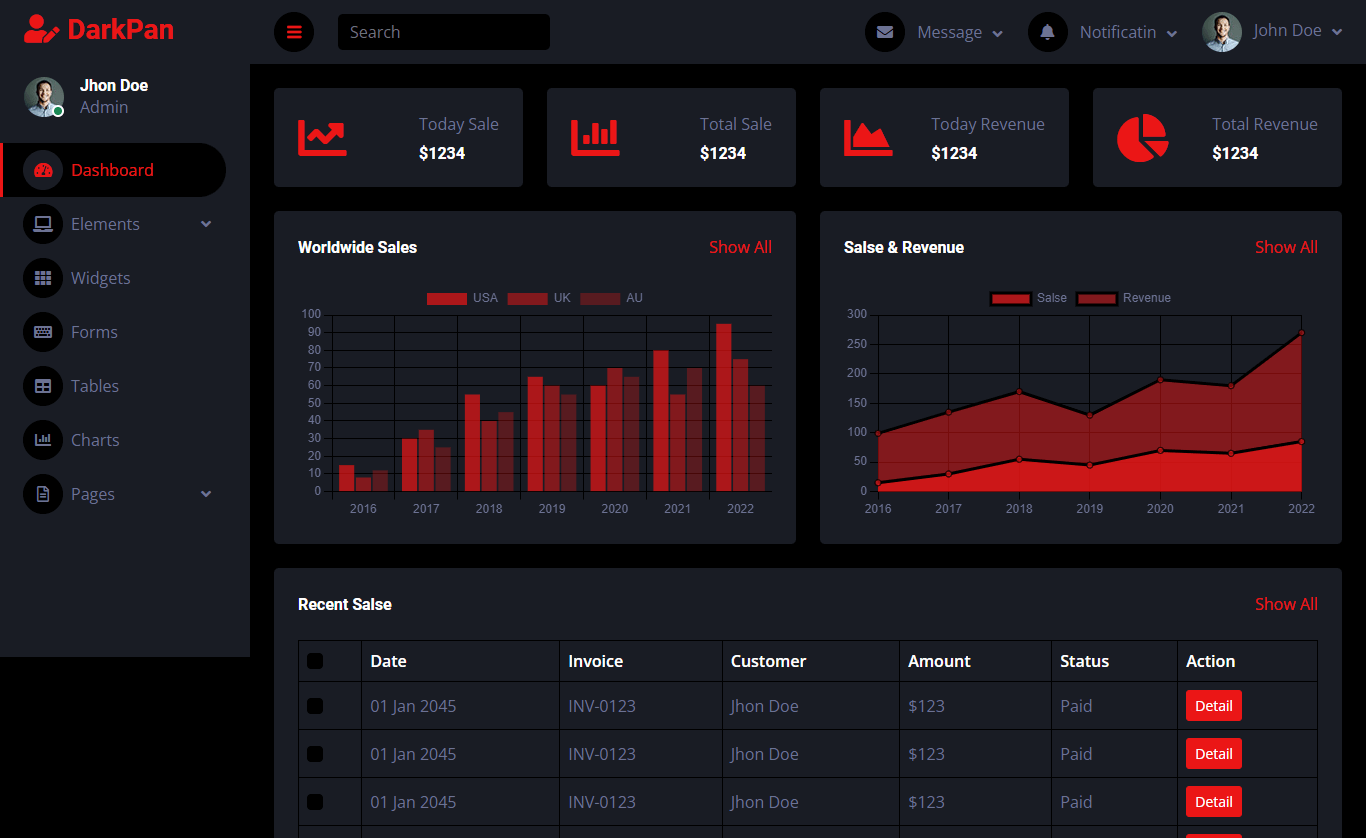
\includegraphics{img/Darkpen.png}
\caption{}
\end{figure}

    \subsection{Use AJAX}\label{use-ajax}

AJAX, which stands for \textbf{Asynchronous JavaScript and XML}, is a
web development technique that allows web pages to communicate with a
server asynchronously without requiring a full page reload. This means
that specific parts of a web page can be updated dynamically in the
background, while the rest of the page remains unchanged. AJAX is not a
single technology but a combination of several technologies, including
\textbf{JavaScript}, \textbf{XML} (or JSON, which is more commonly used
today), \textbf{HTML}, and \textbf{CSS}. JavaScript is used to send and
receive data from the server, while XML or JSON formats are used to
structure the data being exchanged. The key advantage of AJAX is that it
enhances user experience by making web applications faster and more
interactive, as users can interact with the page without interruptions
caused by full page reloads. For example, when you type a search query
into Google, the suggestions that appear dynamically are powered by
AJAX. Similarly, AJAX is widely used in features like live form
validation, auto-complete, and real-time updates in social media feeds.
By enabling asynchronous communication, AJAX reduces server load and
bandwidth usage, making web applications more efficient and responsive.

\subsection{Use AI}\label{use-ai}

We can use AI to write a simple code faster

\begin{Shaded}
\begin{Highlighting}[]
  \KeywordTok{function} \AttributeTok{fetchData}\NormalTok{() }\OperatorTok{\{}
    \AttributeTok{fetch}\NormalTok{(}\StringTok{'posts/1'}\NormalTok{) }\CommentTok{// URL of the Python server}
\NormalTok{       .}\AttributeTok{then}\NormalTok{(response }\OperatorTok{=>} \OperatorTok{\{}
         \ControlFlowTok{if}\NormalTok{ (}\OperatorTok{!}\VariableTok{response}\NormalTok{.}\AttributeTok{ok}\NormalTok{) }\OperatorTok{\{}
              \ControlFlowTok{throw} \KeywordTok{new} \AttributeTok{Error}\NormalTok{(}\StringTok{'Network response was not ok'}\NormalTok{)}\OperatorTok{;}
              \OperatorTok{\}}
           \ControlFlowTok{return} \VariableTok{response}\NormalTok{.}\AttributeTok{json}\NormalTok{()}\OperatorTok{;}
           \OperatorTok{\}}\NormalTok{)}
\NormalTok{         .}\AttributeTok{then}\NormalTok{(data }\OperatorTok{=>} \OperatorTok{\{}
         \CommentTok{//add data to chart}
         \AttributeTok{addData}\NormalTok{(lab}\OperatorTok{,}\VariableTok{data}\NormalTok{.}\AttributeTok{val}\NormalTok{[}\DecValTok{0}\NormalTok{]}\OperatorTok{,}\VariableTok{data}\NormalTok{.}\AttributeTok{val}\NormalTok{[}\DecValTok{1}\NormalTok{])}\OperatorTok{;}
\NormalTok{         lab }\OperatorTok{=}\NormalTok{ lab}\OperatorTok{+}\DecValTok{1}\OperatorTok{;}
         \CommentTok{//show data in label }
         \VariableTok{document}\NormalTok{.}\AttributeTok{getElementById}\NormalTok{(}\StringTok{'result'}\NormalTok{).}\AttributeTok{innerHTML} \OperatorTok{=} \VerbatimStringTok{`}
\VerbatimStringTok{          <h2>Title: }\SpecialCharTok{$\{}\VariableTok{data}\NormalTok{.}\AttributeTok{title}\SpecialCharTok{\}}\VerbatimStringTok{</h2>}
\VerbatimStringTok{          <p>Body: }\SpecialCharTok{$\{}\VariableTok{data}\NormalTok{.}\AttributeTok{val}\SpecialCharTok{\}}\VerbatimStringTok{</p>}
\VerbatimStringTok{              `}\OperatorTok{;}
           \OperatorTok{\}}\NormalTok{)}
\NormalTok{          .}\AttributeTok{catch}\NormalTok{(error }\OperatorTok{=>} \OperatorTok{\{}
  \VariableTok{document}\NormalTok{.}\AttributeTok{getElementById}\NormalTok{(}\StringTok{'result'}\NormalTok{).}\AttributeTok{innerHTML} \OperatorTok{=} \StringTok{'Error fetching data'}\OperatorTok{;}
                \OperatorTok{\}}\NormalTok{)}\OperatorTok{;}
    \OperatorTok{\};}
\end{Highlighting}
\end{Shaded}

    \subsection{Use Timer in JS}\label{use-timer-in-js}

\begin{Shaded}
\begin{Highlighting}[]
\AttributeTok{setInterval}\NormalTok{(fetchData}\OperatorTok{,} \DecValTok{1500}\NormalTok{)}\OperatorTok{;}
\end{Highlighting}
\end{Shaded}

    \subsection{chart in JS}\label{chart-in-js}

\textbf{Chart.js} is a popular open-source JavaScript library used for
creating responsive, interactive, and visually appealing charts and
graphs on web pages. It is lightweight, easy to use, and highly
customizable, making it a go-to choice for developers who need to
visualize data in their web applications. Chart.js supports a wide
variety of chart types, including bar charts, line charts, pie charts,
doughnut charts, radar charts, polar area charts, and more. The library
uses HTML5's \texttt{\textless{}canvas\textgreater{}} element to render
charts, ensuring smooth performance and compatibility with modern
browsers. One of the key features of Chart.js is its
simplicity---developers can create charts with just a few lines of code
by defining datasets, labels, and configuration options. Additionally,
Chart.js is highly interactive; users can hover over data points to see
tooltips, click to highlight sections, or even animate charts for a
dynamic experience. The library also supports responsiveness, meaning
charts automatically adjust to fit different screen sizes, making them
ideal for both desktop and mobile applications. With its extensive
documentation, active community, and flexibility, Chart.js is a powerful
tool for data visualization in web development.

\texttt{javascript\ \ \ \ function\ addData(label,\ data1,data2)\ \{\ \ \ \ \ \ window.myChart2.data.labels.push(label);\ //\ Add\ the\ new\ label\ \ \ \ \ \ window.myChart2.data.datasets{[}0{]}.data.push(data1);\ \ \ \ \ \ window.myChart2.data.datasets{[}1{]}.data.push(data2);\ \ \ \ \ \ window.myChart2.update();\ //\ Update\ the\ chart\ \ \ \ \}}

    \section{Hardware}\label{hardware}

In this project, an attempt has been made to use symbolic data for
display on the web. In this minimal hardware setup, the XADC sensor is
used to read the processor temperature and core voltage. Additionally,
to demonstrate that the XADC is directly accessible from within the PS
(Processing System), no bitstream was used, and the project was even
built without the need for the VIVADO project.

Several objectives have been pursued in reading the sensors:

\begin{enumerate}
\def\labelenumi{\arabic{enumi}.}
\tightlist
\item
  \textbf{Using XADC directly without an IP core in the PL (Programmable
  Logic)}.\\
\item
  \textbf{Demonstrating the drivers provided for XADC within Linux}.\\
\item
  \textbf{Connecting Python to Linux drivers and reading data}.
\end{enumerate}

\subsection{XADC Driver in Linux}\label{xadc-driver-in-linux}

driver address for xadc is \textbf{/sys/bus/iio/devices/iio:device0/}

    \begin{Verbatim}[commandchars=\\\{\}]
{\color{incolor}In [{\color{incolor}15}]:} \PY{o}{!}ls /sys/bus/iio/devices/iio:device0/
\end{Verbatim}


    \begin{Verbatim}[commandchars=\\\{\}]
dev			  in\_voltage2\_vccbram\_raw    in\_voltage6\_vrefp\_scale
events			  in\_voltage2\_vccbram\_scale  in\_voltage7\_vrefn\_raw
in\_temp0\_offset		  in\_voltage3\_vccpint\_raw    in\_voltage7\_vrefn\_scale
in\_temp0\_raw		  in\_voltage3\_vccpint\_scale  name
in\_temp0\_scale		  in\_voltage4\_vccpaux\_raw    of\_node
in\_voltage0\_vccint\_raw	  in\_voltage4\_vccpaux\_scale  power
in\_voltage0\_vccint\_scale  in\_voltage5\_vccoddr\_raw    sampling\_frequency
in\_voltage1\_vccaux\_raw	  in\_voltage5\_vccoddr\_scale  subsystem
in\_voltage1\_vccaux\_scale  in\_voltage6\_vrefp\_raw      uevent

    \end{Verbatim}

    for example reading adc raw data for temperature is:

    \begin{Verbatim}[commandchars=\\\{\}]
{\color{incolor}In [{\color{incolor}16}]:} \PY{o}{!}cat /sys/bus/iio/devices/iio:device0/in\PYZus{}temp0\PYZus{}raw
\end{Verbatim}


    \begin{Verbatim}[commandchars=\\\{\}]
2696

    \end{Verbatim}

    \[ temperature = \frac{RawData * 503.975}{4096} -273\]

    Taksun Simple Web Server 

    \section{web server sample code for
backend}\label{web-server-sample-code-for-backend}

\subsection{Import linrary}\label{import-linrary}

    \begin{Verbatim}[commandchars=\\\{\}]
{\color{incolor}In [{\color{incolor}1}]:} \PY{k+kn}{from} \PY{n+nn}{http}\PY{n+nn}{.}\PY{n+nn}{server} \PY{k}{import} \PY{n}{SimpleHTTPRequestHandler}\PY{p}{,} \PY{n}{HTTPServer}
        \PY{k+kn}{from} \PY{n+nn}{urllib}\PY{n+nn}{.}\PY{n+nn}{parse} \PY{k}{import} \PY{n}{urlparse}\PY{p}{,} \PY{n}{parse\PYZus{}qs}
        \PY{k+kn}{import} \PY{n+nn}{threading}
        \PY{k+kn}{import} \PY{n+nn}{json}
\end{Verbatim}


    \subsection{Read data from XADC driver in
python}\label{read-data-from-xadc-driver-in-python}

    \begin{Verbatim}[commandchars=\\\{\}]
{\color{incolor}In [{\color{incolor}2}]:} \PY{k}{def} \PY{n+nf}{read\PYZus{}xadc\PYZus{}temperature}\PY{p}{(}\PY{p}{)}\PY{p}{:}
            \PY{k}{try}\PY{p}{:}
                \PY{k}{with} \PY{n+nb}{open}\PY{p}{(}\PY{l+s+s2}{\PYZdq{}}\PY{l+s+s2}{/sys/bus/iio/devices/iio:device0/in\PYZus{}temp0\PYZus{}raw}\PY{l+s+s2}{\PYZdq{}}\PY{p}{,} \PY{l+s+s2}{\PYZdq{}}\PY{l+s+s2}{r}\PY{l+s+s2}{\PYZdq{}}\PY{p}{)} \PY{k}{as} \PY{n}{raw\PYZus{}file}\PY{p}{,} \PYZbs{}
                     \PY{n+nb}{open}\PY{p}{(}\PY{l+s+s2}{\PYZdq{}}\PY{l+s+s2}{/sys/bus/iio/devices/iio:device0/in\PYZus{}voltage0\PYZus{}vccint\PYZus{}scale}\PY{l+s+s2}{\PYZdq{}}\PY{p}{,} \PY{l+s+s2}{\PYZdq{}}\PY{l+s+s2}{r}\PY{l+s+s2}{\PYZdq{}}\PY{p}{)} \PY{k}{as} \PY{n}{scale\PYZus{}file}\PY{p}{,}\PYZbs{}
                     \PY{n+nb}{open}\PY{p}{(}\PY{l+s+s2}{\PYZdq{}}\PY{l+s+s2}{/sys/bus/iio/devices/iio:device0/in\PYZus{}voltage0\PYZus{}vccint\PYZus{}raw}\PY{l+s+s2}{\PYZdq{}}\PY{p}{,} \PY{l+s+s2}{\PYZdq{}}\PY{l+s+s2}{r}\PY{l+s+s2}{\PYZdq{}}\PY{p}{)} \PY{k}{as} \PY{n}{vcore\PYZus{}file}\PY{p}{:}
                    \PY{n}{raw} \PY{o}{=} \PY{n+nb}{int}\PY{p}{(}\PY{n}{raw\PYZus{}file}\PY{o}{.}\PY{n}{read}\PY{p}{(}\PY{p}{)}\PY{o}{.}\PY{n}{strip}\PY{p}{(}\PY{p}{)}\PY{p}{)}
                    \PY{n}{scale} \PY{o}{=} \PY{n+nb}{float}\PY{p}{(}\PY{n}{scale\PYZus{}file}\PY{o}{.}\PY{n}{read}\PY{p}{(}\PY{p}{)}\PY{o}{.}\PY{n}{strip}\PY{p}{(}\PY{p}{)}\PY{p}{)}
                    \PY{n}{core} \PY{o}{=} \PY{n+nb}{int}\PY{p}{(}\PY{n}{vcore\PYZus{}file}\PY{o}{.}\PY{n}{read}\PY{p}{(}\PY{p}{)}\PY{o}{.}\PY{n}{strip}\PY{p}{(}\PY{p}{)}\PY{p}{)} 
                    \PY{n}{temp} \PY{o}{=} \PY{p}{(}\PY{n}{raw} \PY{o}{*}\PY{l+m+mf}{503.975}\PY{o}{/}\PY{l+m+mi}{4096}\PY{p}{)} \PY{o}{\PYZhy{}}\PY{l+m+mi}{273}
                    \PY{n}{vcore} \PY{o}{=} \PY{n}{scale} \PY{o}{*} \PY{n}{core}\PY{p}{;}
                    \PY{k}{return} \PY{p}{[}\PY{n}{temp}\PY{p}{,}\PY{n}{vcore}\PY{p}{]}
            \PY{k}{except} \PY{n+ne}{Exception} \PY{k}{as} \PY{n}{e}\PY{p}{:}
                \PY{n+nb}{print}\PY{p}{(}\PY{n}{f}\PY{l+s+s2}{\PYZdq{}}\PY{l+s+s2}{Error reading XADC temperature: }\PY{l+s+si}{\PYZob{}e\PYZcb{}}\PY{l+s+s2}{\PYZdq{}}\PY{p}{)}
                \PY{k}{return} \PY{k+kc}{None}
\end{Verbatim}


    \subsection{Override HTTP Handler
method}\label{override-http-handler-method}

    \begin{Verbatim}[commandchars=\\\{\}]
{\color{incolor}In [{\color{incolor} }]:} \PY{k}{class} \PY{n+nc}{MyHandler}\PY{p}{(}\PY{n}{SimpleHTTPRequestHandler}\PY{p}{)}\PY{p}{:}
            \PY{k}{def} \PY{n+nf}{do\PYZus{}GET}\PY{p}{(}\PY{n+nb+bp}{self}\PY{p}{)}\PY{p}{:}
                \PY{k}{if} \PY{n+nb+bp}{self}\PY{o}{.}\PY{n}{path} \PY{o}{==} \PY{l+s+s1}{\PYZsq{}}\PY{l+s+s1}{/posts/1}\PY{l+s+s1}{\PYZsq{}}\PY{p}{:}
                    \PY{n}{posts} \PY{o}{=} \PY{p}{\PYZob{}}
                        \PY{l+m+mi}{1}\PY{p}{:} \PY{p}{\PYZob{}}
                            \PY{l+s+s2}{\PYZdq{}}\PY{l+s+s2}{id}\PY{l+s+s2}{\PYZdq{}}\PY{p}{:} \PY{l+m+mi}{1}\PY{p}{,}
                            \PY{l+s+s2}{\PYZdq{}}\PY{l+s+s2}{title}\PY{l+s+s2}{\PYZdq{}}\PY{p}{:} \PY{l+s+s2}{\PYZdq{}}\PY{l+s+s2}{temp}\PY{l+s+s2}{\PYZdq{}}\PY{p}{,}
                            \PY{l+s+s2}{\PYZdq{}}\PY{l+s+s2}{val}\PY{l+s+s2}{\PYZdq{}}\PY{p}{:} \PY{n}{read\PYZus{}xadc\PYZus{}temperature}\PY{p}{(}\PY{p}{)}
                            \PY{p}{\PYZcb{}}
                            \PY{p}{\PYZcb{}}
                    \PY{n+nb+bp}{self}\PY{o}{.}\PY{n}{send\PYZus{}response}\PY{p}{(}\PY{l+m+mi}{200}\PY{p}{)}  \PY{c+c1}{\PYZsh{} OK}
                    \PY{n+nb+bp}{self}\PY{o}{.}\PY{n}{send\PYZus{}header}\PY{p}{(}\PY{l+s+s1}{\PYZsq{}}\PY{l+s+s1}{Content\PYZhy{}type}\PY{l+s+s1}{\PYZsq{}}\PY{p}{,} \PY{l+s+s1}{\PYZsq{}}\PY{l+s+s1}{application/json}\PY{l+s+s1}{\PYZsq{}}\PY{p}{)}
                    \PY{n+nb+bp}{self}\PY{o}{.}\PY{n}{end\PYZus{}headers}\PY{p}{(}\PY{p}{)}
                    \PY{n}{response} \PY{o}{=} \PY{n}{json}\PY{o}{.}\PY{n}{dumps}\PY{p}{(}\PY{n}{posts}\PY{p}{[}\PY{l+m+mi}{1}\PY{p}{]}\PY{p}{)}\PY{o}{.}\PY{n}{encode}\PY{p}{(}\PY{l+s+s1}{\PYZsq{}}\PY{l+s+s1}{utf\PYZhy{}8}\PY{l+s+s1}{\PYZsq{}}\PY{p}{)}
                    \PY{n+nb+bp}{self}\PY{o}{.}\PY{n}{wfile}\PY{o}{.}\PY{n}{write}\PY{p}{(}\PY{n}{response}\PY{p}{)}
        
                \PY{k}{else}\PY{p}{:}
                    \PY{n+nb}{super}\PY{p}{(}\PY{p}{)}\PY{o}{.}\PY{n}{do\PYZus{}GET}\PY{p}{(}\PY{p}{)}
        
            \PY{k}{def} \PY{n+nf}{log\PYZus{}message}\PY{p}{(}\PY{n+nb+bp}{self}\PY{p}{,} \PY{n+nb}{format}\PY{p}{,} \PY{o}{*}\PY{n}{args}\PY{p}{)}\PY{p}{:}
                \PY{k}{pass}
        
            \PY{k}{def} \PY{n+nf}{log\PYZus{}request}\PY{p}{(}\PY{n+nb+bp}{self}\PY{p}{,} \PY{n+nb}{format}\PY{p}{,} \PY{o}{*}\PY{n}{args}\PY{p}{)}\PY{p}{:}
                \PY{k}{pass}
\end{Verbatim}


    \subsection{Function for running
server}\label{function-for-running-server}

    \begin{Verbatim}[commandchars=\\\{\}]
{\color{incolor}In [{\color{incolor}4}]:} \PY{k}{def} \PY{n+nf}{run\PYZus{}server}\PY{p}{(}\PY{p}{)}\PY{p}{:}
            \PY{n}{PORT} \PY{o}{=} \PY{l+m+mi}{8000}
            \PY{n}{server\PYZus{}address} \PY{o}{=} \PY{p}{(}\PY{l+s+s1}{\PYZsq{}}\PY{l+s+s1}{\PYZsq{}}\PY{p}{,} \PY{n}{PORT}\PY{p}{)}
            \PY{n}{httpd} \PY{o}{=} \PY{n}{HTTPServer}\PY{p}{(}\PY{n}{server\PYZus{}address}\PY{p}{,} \PY{n}{MyHandler}\PY{p}{)}
            \PY{n+nb}{print}\PY{p}{(}\PY{n}{f}\PY{l+s+s2}{\PYZdq{}}\PY{l+s+s2}{Serving on port }\PY{l+s+si}{\PYZob{}PORT\PYZcb{}}\PY{l+s+s2}{...}\PY{l+s+s2}{\PYZdq{}}\PY{p}{)}
            \PY{n}{httpd}\PY{o}{.}\PY{n}{serve\PYZus{}forever}\PY{p}{(}\PY{p}{)}
\end{Verbatim}


    \subsection{Run server function in
theread}\label{run-server-function-in-theread}

    \begin{Verbatim}[commandchars=\\\{\}]
{\color{incolor}In [{\color{incolor}5}]:} \PY{n}{server\PYZus{}thread} \PY{o}{=} \PY{n}{threading}\PY{o}{.}\PY{n}{Thread}\PY{p}{(}\PY{n}{target}\PY{o}{=}\PY{n}{run\PYZus{}server}\PY{p}{)}
        \PY{n}{server\PYZus{}thread}\PY{o}{.}\PY{n}{daemon} \PY{o}{=} \PY{k+kc}{True}  
        \PY{n}{server\PYZus{}thread}\PY{o}{.}\PY{n}{start}\PY{p}{(}\PY{p}{)}
\end{Verbatim}



    % Add a bibliography block to the postdoc
    
    
    
    \end{document}
